\section{Filter}
Die Filter-Charakteristik kann mithilfe der Übertragungsfunktion $H(s)$ beschrieben werden. Dabei sind \textbf{Hochpass}-Filter mit einem Reellen Zähler und \textbf{Tiefpass} mit Imaginären Zähler erkennbar. Das heisst, dass $j\omega = s$ für Hochpassfilter nicht im Zähler vorkommen dürfen.

Die DC-Verstärkung kann bei $H(0) = \text{DC}$ erhausgelesen werden. 

\noindent\textbf{Hochpass}:\\
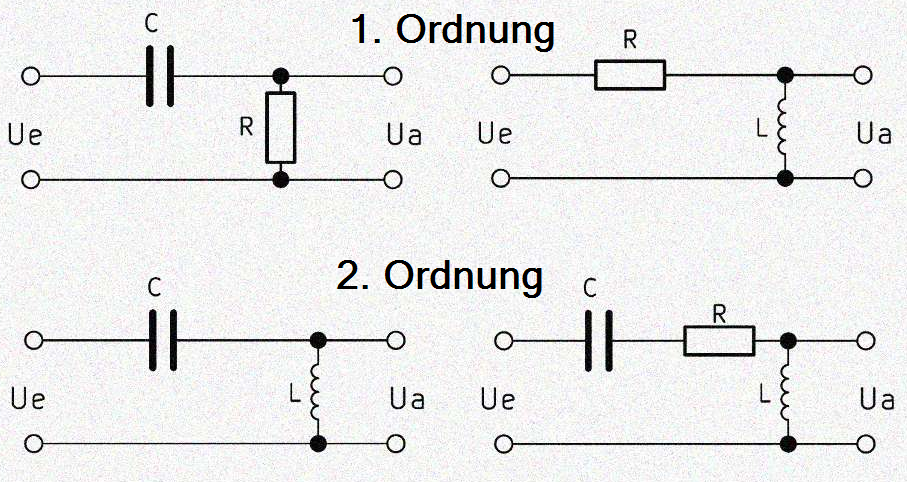
\includegraphics[width=\columnwidth]{Images/hochpass}

\noindent\textbf{Tiefpass}:\\
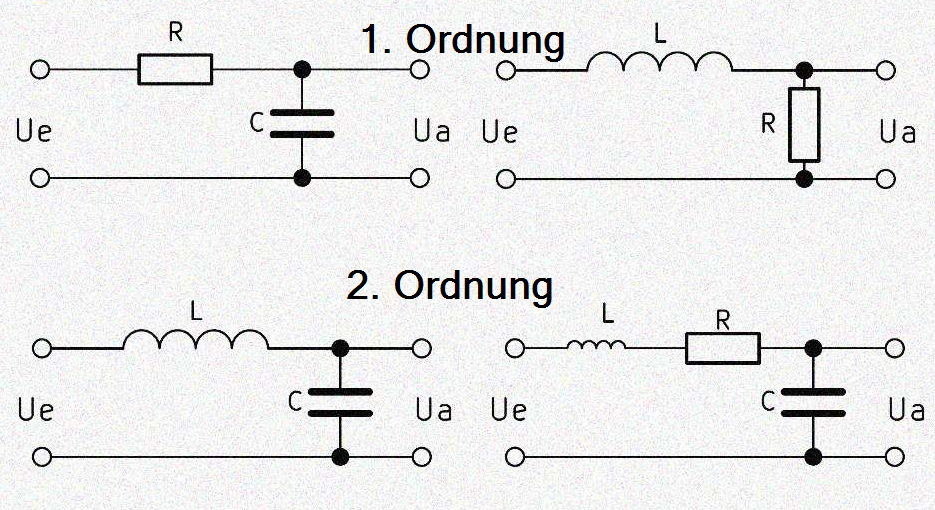
\includegraphics[width=\columnwidth]{Images/tiefpass}


\begin{center}
	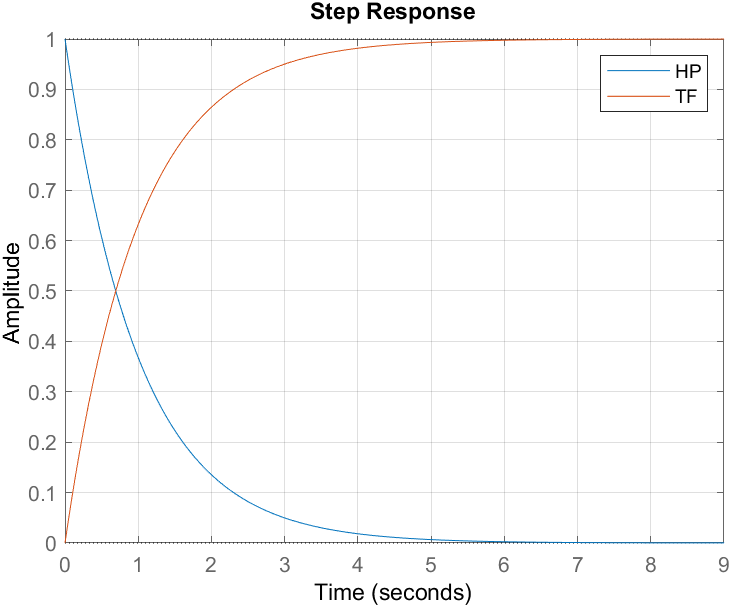
\includegraphics[width=0.49\columnwidth]{Images/stepreponse}
	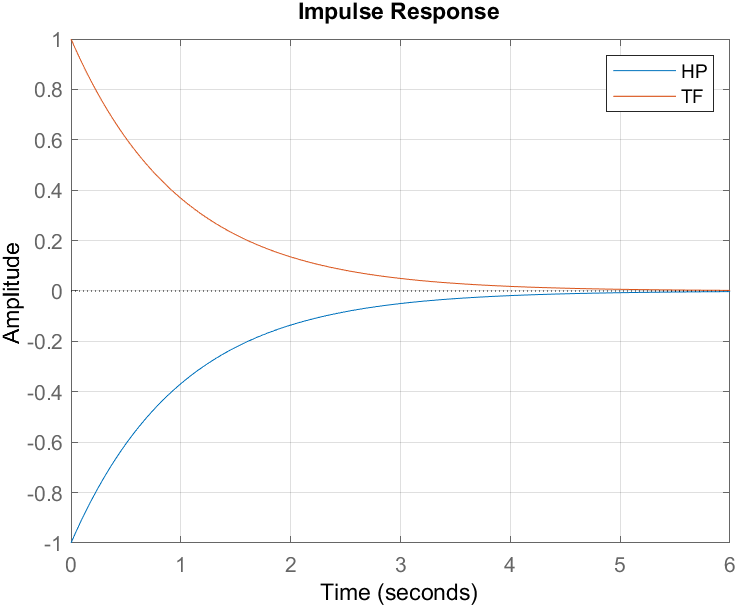
\includegraphics[width=0.49\columnwidth]{Images/impulse}
\end{center}
